\section{Pruebas y Resultados}
El modelo seleccionado, que demostró la mayor eficacia, se basó en la arquitectura MobileNet V3. Esta red neuronal convolucional fue elegida como la red troncal del modelo debido a su capacidad para operar eficientemente en dispositivos con recursos limitados, sin comprometer significativamente el rendimiento. Los resultados obtenidos son altamente prometedores, como se evidencia en las métricas de rendimiento del modelo.  El modelo alcanzó una precisión global del 98.37\%, superando métodos tradicionales como SVM y Random Forest (precisión del 96\% según Díaz, 2023). Esto implica que el modelo es capaz de clasificar correctamente el mas del 98\% de las imágenes probadas. Esta métrica es particularmente importante en aplicaciones prácticas donde la fiabilidad de la clasificación es crítica para el análisis posterior.

El recall obtenido fue de 0.9914, lo que refleja la alta sensibilidad del modelo en la detección de las regiones con presencia de palma de aceite. En términos prácticos, esto significa que el modelo identificó correctamente el 99.14\% de todas las áreas relevantes en el conjunto de datos. Esta tasa de detección es crucial en estudios de cobertura de tierra donde la omisión de áreas significativas puede llevar a conclusiones erróneas.

En cuanto a la precisión, el modelo alcanzó un 99.04\%, indicando que, de las regiones clasificadas como palma de aceite, el 99.04\% efectivamente correspondían a dichos cultivos. Esta alta precisión es indispensable para minimizar los falsos positivos, una métrica especialmente importante cuando se toman decisiones de gestión de tierras basadas en los datos de clasificación.

Finalmente, el F1-score del modelo fue de 0.9909, revelando un equilibrio casi perfecto entre precisión y recall. Esto sugiere que el modelo no solo es altamente confiable en la identificación de áreas de palma de aceite, sino que también mantiene una baja tasa de falsos positivos y negativos, un aspecto fundamental para la integridad del análisis espacial. Estos resultados subrayan la eficacia del modelo MobileNet V3 para la detección de palma de aceite y su aplicabilidad potencial en la monitorización a gran escala de la agricultura y la gestión del uso de la tierra.

\begin{figure*}[t]
 \centering
 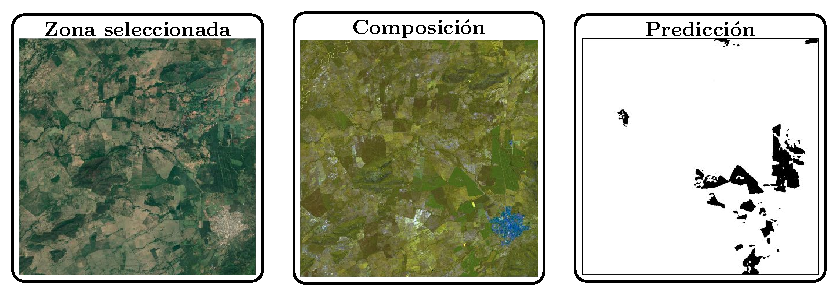
\includegraphics[width=\textwidth]{example_selected_zone}
 \caption{Ejemplo de predicción del modelo sobre un área con cultivos}
 \label{fig:example_selected_zone}
\end{figure*}

En la Figura \ref{fig:example_selected_zone} podemos ver una zona seleccionada de 10x10 km de Colombia, seguido de la composición de Sentinel 1 y Sentinel 2 y por último tenemos la salida del modelo la en la cual la clase 1 es la que esta en negro donde el modelo clasifica que hay palma de aceite mientras que donde en la mascara donde esta en blanco el modelo indica que no hay palma de aceite en esta imagen.

\begin{figure*}[t]
 \centering
 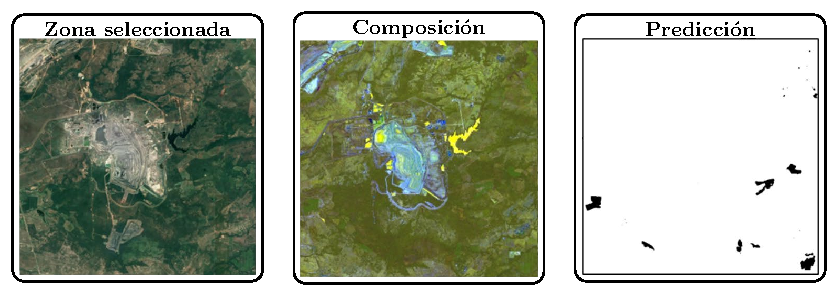
\includegraphics[width=\textwidth]{example_few_crops}
 \caption{Ejemplo de predicción del modelo sobre un área con pocos cultivos}
 \label{fig:example_few_crops}
\end{figure*}

En la Figura \ref{fig:example_few_crops}, podemos observar una zona de explotación minera que, en la composición, adquiere un color celeste. Además, se identifica un cuerpo de agua que adopta un color amarillo en la composición. Por otra parte, tenemos las plantaciones de palma de aceite, las cuales presentan un color verde distintivo. En esta zona seleccionada, los cultivos de palma de aceite son escasos, motivo por el cual el color verde no es tan predominante en la imagen. En la máscara predicha por el modelo, podemos observar que se clasifican correctamente las zonas que contienen plantaciones de palma de aceite.

\begin{figure*}[t]
 \centering
 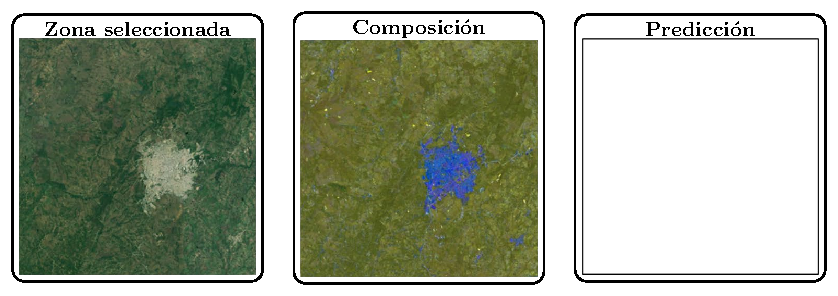
\includegraphics[width=\textwidth]{example_without_crops}
 \caption{Ejemplo de predicción del modelo sobre área sin cultivos}
 \label{fig:example_without_crops}
\end{figure*}

En la Figura \ref{fig:example_without_crops} se seleccionó una zona donde no hay presencia de palma de aceite y, además, existe una área metropolitana. En este caso, se puede observar que el modelo devuelve una máscara completamente blanca, indicando que el modelo clasifica correctamente la ausencia de cultivos de palma de aceite en esta zona.

\begin{figure*}[t]
 \centering
 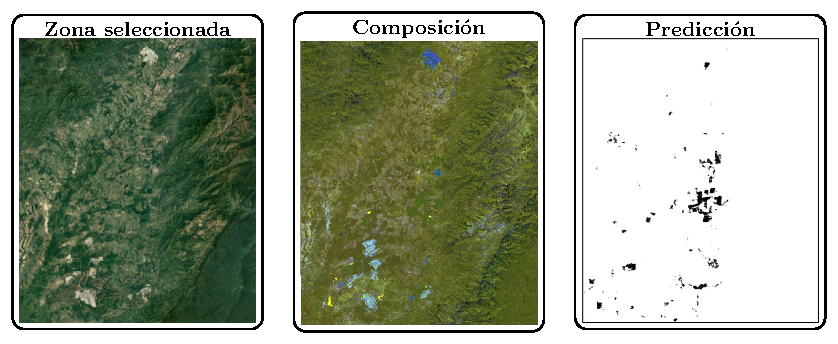
\includegraphics[width=\textwidth]{full_prediction}
 \caption{Predicción del modelo sobre toda la zona seleccionada}
 \label{fig:full_prediction}
\end{figure*}

En la Figura \ref{fig:full_prediction} se presenta la zona seleccionada en su totalidad, donde se encuentran áreas metropolitanas, bosques, diversas plantaciones de otros cultivos, además de zonas rocosas y una gran diversidad de flora. A continuación, se muestra la predicción, en la que las áreas en negro representan las regiones que el modelo de clasificación ha identificado como contenedoras de palma de aceite. El color blanco representa áreas donde el modelo predice la ausencia de palma de aceite.

\begin{figure}
 \centering
 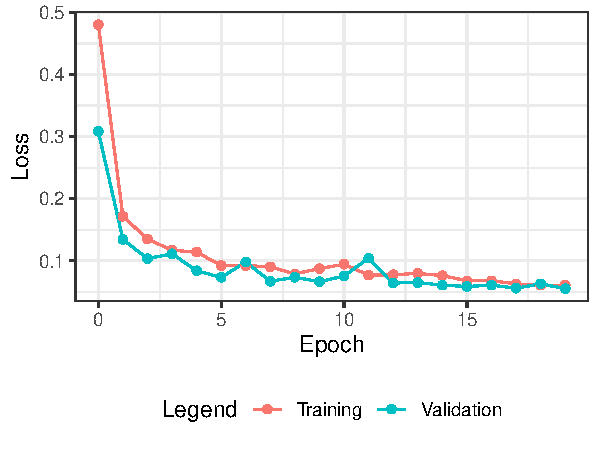
\includegraphics[width=\columnwidth]{loss}
 \caption{Gráfica de perdida (loss)}
 \label{fig:loss}
\end{figure}

\begin{figure}
 \centering
 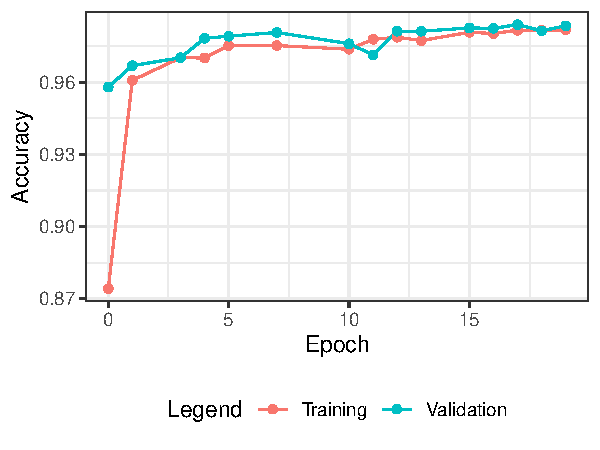
\includegraphics[width=\columnwidth]{accuracy}
 \caption{Gráfica de exactitud (accuracy)}
 \label{fig:accuracy}
\end{figure}

En el gráfico que se muestra en la Figura \ref{fig:loss}, se muestra la pérdida de entrenamiento y validación. Se observa una disminución rápida de la pérdida en las primeras épocas, seguida de una estabilización, lo que sugiere que el modelo rápidamente alcanzó un punto de convergencia. De manera similar, en el gráfico \ref{fig:accuracy}, las líneas representan la precisión de entrenamiento y validación, ambas alcanzando valores superiores al 90\% y manteniéndose relativamente constantes después de las primeras épocas, lo que indica un buen ajuste del modelo.

\begin{figure}
 \centering
 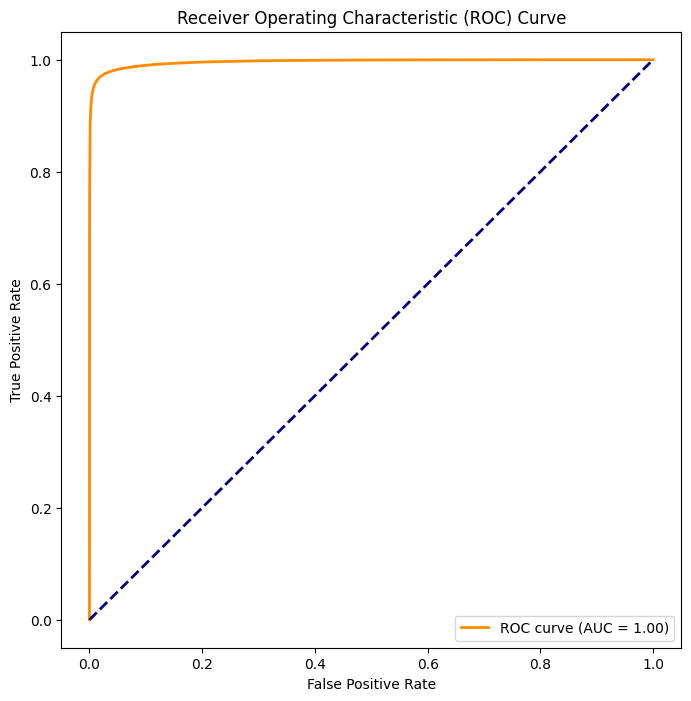
\includegraphics[width=0.8\columnwidth]{roc}
 \caption{Curva ROC del modelo}
 \label{fig:roc}
\end{figure}


La figura Figura \ref{fig:roc} representa la Curva Característica de Operación del Receptor (ROC) con un área bajo la curva (AUC) de 1.00. La curva ROC es una línea naranja que se adhiere perfectamente al borde superior izquierdo del gráfico, lo cual es indicativo de un rendimiento excepcional del modelo, ya que demuestra una tasa de verdaderos positivos del 100\% a lo largo de todos los umbrales de clasificación, con una tasa de falsos positivos que se mantiene en cero. El gráfico también incluye una línea punteada azul que representa el rendimiento de un clasificador aleatorio, lo que resalta aún más la superioridad del modelo en cuestión.

Por último, haciendo una comparación con el modelo presentado por \cite{diaz2023} en la que se utilizaron una variedad de algoritmos de aprendizaje automático más tradicionales, como regresión logística, Random Forest, SVM y XGBoost. Aunque estos métodos son eficaces y versátiles, pueden no ser tan específicos como los modelos de Deep Learning para tareas detalladas de segmentación de imágenes. Además, Díaz incorporó índices de vegetación y variables de textura en su análisis, lo que indica un enfoque en aspectos específicos de la vegetación y el terreno. Aunque esta metodología es útil, posiblemente no captura la gama completa de características que se pueden obtener con el enfoque del usuario. La precisión del modelo de Díaz fue ligeramente inferior, con un 96\%, lo que sugiere que los enfoques más tradicionales de aprendizaje automático pueden siguen siendo efectivos para tareas de clasificación detalladas en comparación con métodos avanzados de Deep Learning.
